\documentclass[12pt, a4paper, twoside]{article}

%% Preamble
\usepackage{pdfpages}           % Para incluir PDFs
\usepackage{graphicx}           % Para gráficos
\usepackage{subfiles}           % Para manejar subarchivos
\usepackage{hyperref}           % Para enlaces
\usepackage{listings}           % Para código fuente (ajusta lenguaje)
\usepackage{verbatim}
\usepackage[backend=bibtex,style=numeric]{biblatex} % Para citas numéricas
\addbibresource{references.bib} % Cargar archivo .bib
\usepackage{url}
\usepackage{float}


\usepackage{geometry}           % Para ajustar márgenes

% Ajustes de márgenes
\geometry{
	left=3cm,       % Margen izquierdo
	right=3cm,      % Margen derecho
	top=2.5cm,      % Margen superior
	bottom=2.5cm,   % Margen inferior
	headheight=15pt, % Altura del encabezado
	twoside          % Para documentos a dos caras
}


\graphicspath{{images/}{../images/}} % Ruta para imágenes

\begin{document}
	
	%% Cover
	
\includepdf[noautoscale=true, width=\paperwidth]{cover.pdf}
	
	%% Title
	\clearpage
	\setcounter{page}{1}
	
\includepdf[noautoscale=true, width=\paperwidth]{title.pdf}
	
	%%%%%%%%%%%%%%%%%%%%%%%%%%%%%%%%%%%%%%%%%%%%%%%%%%%%%%%%%%%%%%%%%%%%%%%%%%%
	
	% Índice automático
	\tableofcontents
	\newpage
	
	\section{Introducción}
	
	Este documento es una continuación de las fases anteriores del proyecto, donde se desarrollaron el \textbf{diseño conceptual y lógico} de un almacén de datos basado en la información proporcionada por la \textit{Base de Datos de Investigación Colaborativa eICU} \cite{eICU2024}, y la \textbf{integración de datos} mediante un proceso de Extracción, Transformación y Carga (ETL). Para la creación de un almacén enfocado a \textbf{pacientes con patologías respiratorias}.
	
	En esta fase, se busca construir un \textbf{cubo multidimensional} utilizando los datos del almacén previamente desarrollado,	En el ámbito hospitalario, la creación de un cubo multidimensional ofrece ventajas al permitir analizar datos clínicos complejos de manera ágil. Posteriormente se realizarán consultas en \textit{MDX} (Multidimensional Expressions) sobre dicho cubo.  Permitiendo extraer información de manera eficiente al navegar por las dimensiones y medidas del cubo.

	
	Además, se describirán los problemas encontrados durante el desarrollo y las soluciones aplicadas, asegurando que las consultas generen resultados útiles para el análisis de datos.
	
	
	
	\section{Objetivos}
	
	Los objetivos principales de este informe son los siguientes:
	
	\begin{itemize}
		\item Realizar las correcciones pertinentes en el proceso ETL que permitan el desarrollo del cubo muldimensional.
		\item Implementar un cubo multidimensional adaptado para el análisis de \textbf{pacientes con patologías respiratorias}.
		\item Desarrollar al menos 8 consultas en \textit{MDX} que exploren diferentes dimensiones y hechos del cubo, aplicando funciones avanzadas cuando sea necesario.
		\item Documentar de manera clara y replicable el proceso de creación del cubo multidimensional y las consultas \textit{MDX}, proporcionando instrucciones detalladas para su ejecución.
		\item Describir los problemas encontrados durante el desarrollo del cubo y las consultas, y detallar las soluciones empleadas.
	\end{itemize}
	
	
	 
	
	\section{\textbf{Modificación del almacén de datos}}
	
	\begin{itemize}
		\item Se \textbf{eliminaron las columnas} `Age` y `PatientUnitStayID` de la tabla de pacientes.
		\item Se \textbf{seleccionaron únicamente los pacientes únicos}, conservando solo su primera aparición en la base de datos. Anteriormente, el número total de pacientes era 1849, pero después de aplicar esta modificación, el total es de 1841, lo que es correcto.
		\item Para el \textbf{tiempo}, se utilizó la cláusula `DISTINCT` para evitar \textbf{fechas duplicadas en el ingreso}.
		\item Para la \textbf{información de diagnóstico}, se extrajo el primer valor de la columna `DiagnosisString` (primera dimensión). La consulta SQL utilizada para obtener los datos de diagnóstico de la base de datos fue la siguiente:
		\begin{verbatim}
			SELECT 
			DiagnosisID,
			PatientUnitStayID,
			ActiveUponDischarge,
			DiagnosisOffset,
			ICD9Code,
			DiagnosisPriority,
			SUBSTRING(DiagnosisString, 1, CHARINDEX('|'
			, DiagnosisString + '|') - 1) AS FirstDiagnosis
			FROM Diagnosis;
		\end{verbatim}
		\item Se \textbf{corrigió la creación de las tablas intermedias} para las relaciones `NxM`. Anteriormente, se utilizaba como \textbf{origen de datos la tabla `Diagnosis`} de la base de datos en lugar de la del `Data Warehouse`. Posteriormente, se realizaba un \textbf{`lookup` con `IngresoUCI`} utilizando el `patientID\_og`.
		\item Se \textbf{realizó una transformación en la columna `Age`}, cambiando su tipo de dato de `string` a `integer` para permitir su uso en consultas. Durante este proceso, se transformó el valor `'> 89'` a `90` por defecto. La consulta SQL utilizada para obtener los datos de la tabla `Patient` en la base de datos fue la siguiente:
		\begin{verbatim}
			SELECT 
			T.TiempoID,
			P.UniquePID,
			H.HospitalID,
			I.HospitalDischargeOffset,
			I.PatientHealthSystemStayID,
			I.PatientUnitStayID,
			CASE 
			WHEN I.Age = '> 89' THEN 90                      
			-- Cambiar "> 89" por 90
			WHEN ISNUMERIC(I.Age) = 1 THEN CAST(I.Age AS INT) 
			-- Convertir valores numéricos a INT
			ELSE NULL                                       
			-- Manejar otros casos como NULL
			END AS AgeInt
			FROM [eICU Collaborative Research Database].dbo.Patient I
			LEFT JOIN prueba.dbo.Paciente P ON I.uniquePID = P.uniquePID_og
			LEFT JOIN prueba.dbo.Hospital H ON I.HospitalID = H.hospitalID_og
			LEFT JOIN prueba.dbo.Tiempo T 
			ON I.HospitalDischargeYear = T.HospitalDischargeYear 
			AND I.HospitalDischargeTime24 = T.HospitalDischargeTime24;
		\end{verbatim}
	\end{itemize}
	
		
	
\section{\textbf{Creación del cubo}}

\subsection{\textbf{Orígenes de datos}}

Para la \textbf{creación del cubo}, iniciaremos el proceso estableciendo la conexión con nuestra base de datos:

\begin{figure}[H]
	\centering
	
\includegraphics[width=0.5\textwidth]{image/origenDatos}
	\caption{\textbf{Origen de datos}}
	\label{fig:1}
\end{figure}

A continuación, procederemos a \textbf{establecer la conexión con la base de datos}, donde especificaremos el proveedor a utilizar, como se muestra en la Figura \ref{fig:2}. Dado que nuestro servidor se encuentra en el entorno local, se debe indicar únicamente `.` como la dirección del servidor. Es crucial, \textbf{y se debe prestar especial atención}, que la autenticación se configure utilizando \textbf{SQL Server Authentication}. Esto permitirá especificar el nombre de usuario como `sa` y la contraseña asociada, que en este caso será `Almacenes`. Finalmente, seleccionaremos la base de datos correspondiente, que en este escenario es `prueba`, como se ilustra en la Figura \ref{fig:2}.

\begin{figure}[H]
	\centering
	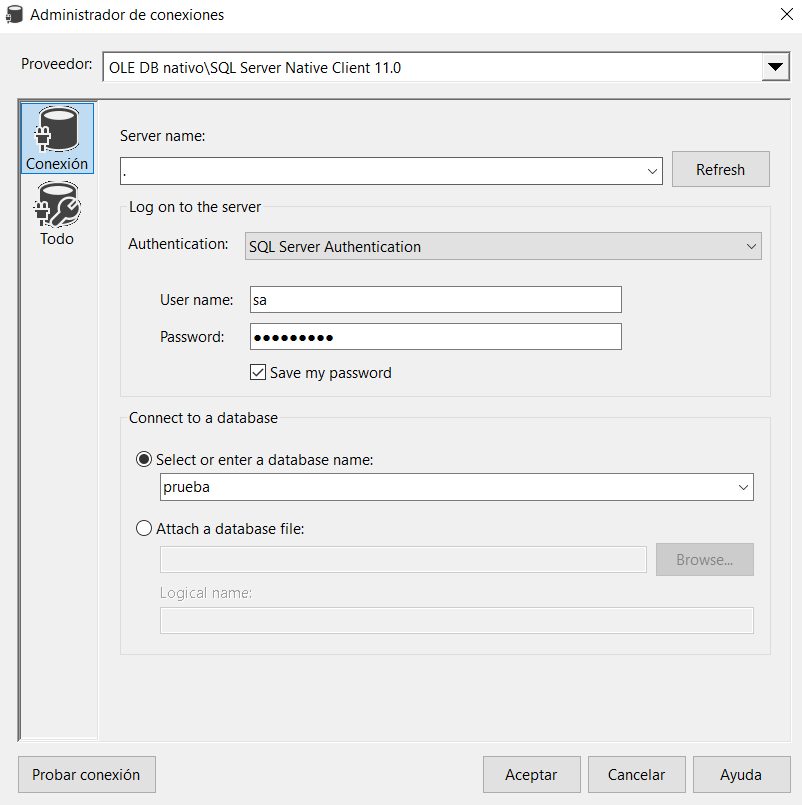
\includegraphics[width=0.8\textwidth]{image/conexion}
	\caption{\textbf{Conexión de datos}}
	\label{fig:2}
\end{figure}

Cabe destacar que en la creación de un cubo se puede seleccionar mejores nombre que "prueba", pero por simplicidad y facilitar el seguimiento de este tutorial, en caso de crear una base de datos se recomendaría usar un nombre más coherente con los datos trabajados, pero al igual que muchos lenguajes de programación se le puede asignar el nombre deseado mientras se mantenga la lógica y la correcta llamada de la misma.

Una vez realizados los pasos anteriores, procederemos a hacer clic derecho sobre las \textbf{vistas del origen de datos} y seleccionaremos la opción "Nueva Vista". Esto nos mostrará todos los orígenes de datos disponibles, siendo en este caso solo la base de datos "Prueba", como se muestra en la Figura \ref{fig:4}.

\begin{figure}[H]
	\centering
	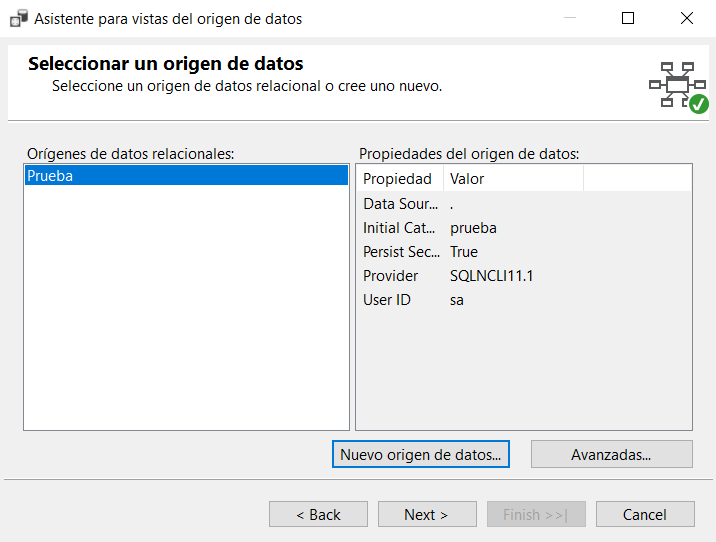
\includegraphics[width=1\textwidth]{image/vistaOrigenConexion}
	\caption{\textbf{Vista origen conexión de datos}}
	\label{fig:4}
\end{figure}

A continuación, procederemos a hacer clic en el botón "Next".

En la pantalla siguiente, tal como se muestra en la Figura \ref{fig:5}, seleccionaremos el \textbf{botón resaltado en rojo}. Esta acción nos permitirá agregar \textbf{todas las tablas a la vista}, lo que es fundamental para asegurar que el almacén de datos incluya toda la información necesaria para la correcta construcción del cubo. Una vez seleccionadas todas las tablas, continuaremos haciendo clic en "Next" para avanzar al siguiente paso del proceso.

\begin{figure}[H]
	\centering
	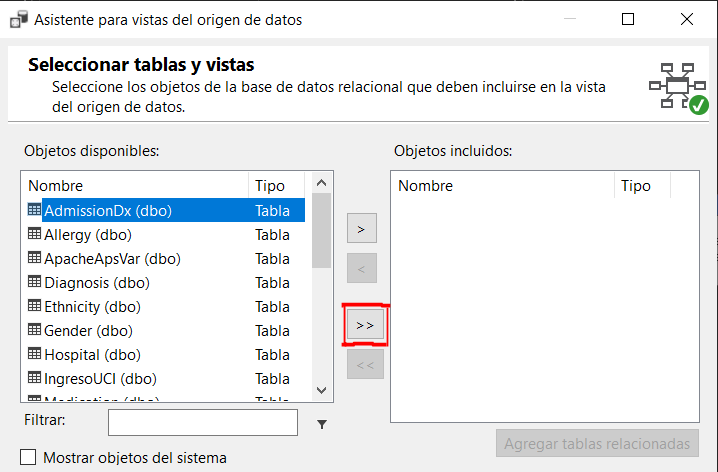
\includegraphics[width=1\textwidth]{image/seleccionTablas}
	\caption{\textbf{Selección de tablas}}
	\label{fig:5}
\end{figure}

Posteriormente, aparecerá una nueva pantalla donde podremos \textbf{visualizar lo que contendrá la vista} y, por ende, con qué elementos podremos operar en el cubo, como se muestra en la Figura \ref{fig:6}.

\begin{figure}[H]
	\centering
	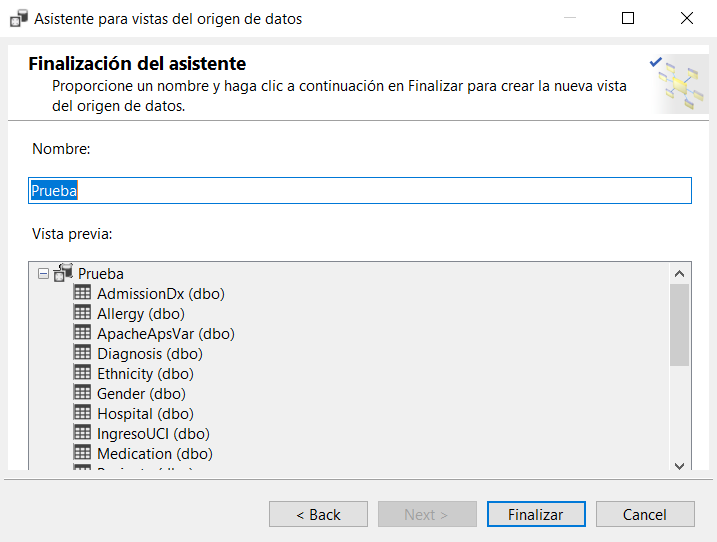
\includegraphics[width=0.7\textwidth]{image/asistenteVista}
	\caption{\textbf{Vista finalización}}
	\label{fig:6}
\end{figure}

Una vez revisado todo, seleccionaremos "Finalizar" como se muestra en la Figura \ref{fig:6}.

Al hacer \textbf{doble clic en la vista recién creada}, podremos ver que contiene todas las tablas que teníamos en nuestro diagrama de SQL Server Management, como se ilustra en la Figura \ref{fig:7}.

\begin{figure}[H]
	\centering
	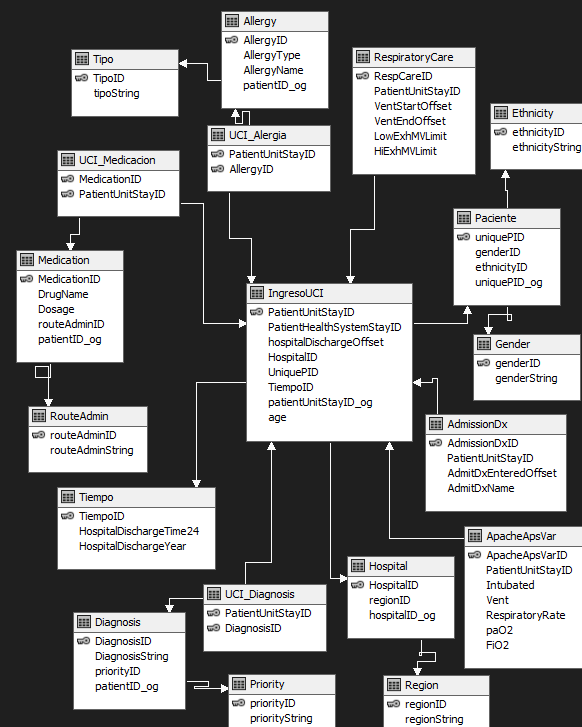
\includegraphics[width=1\textwidth]{image/vista_origenes_datos}
	\caption{\textbf{Vista}}
	\label{fig:7}
\end{figure}

\subsection{\textbf{Crear el cubo}}

Una vez que la \textbf{vista esté configurada}, podemos proceder a \textbf{crear el cubo}. Para ello, haremos clic derecho sobre el proyecto y seleccionaremos "Nuevo Cubo". En la ventana emergente, elegiremos la opción \textbf{"Usar tablas existentes"}, tal como se muestra en la Figura \ref{fig:9}.

\begin{figure}[H]
	\centering
	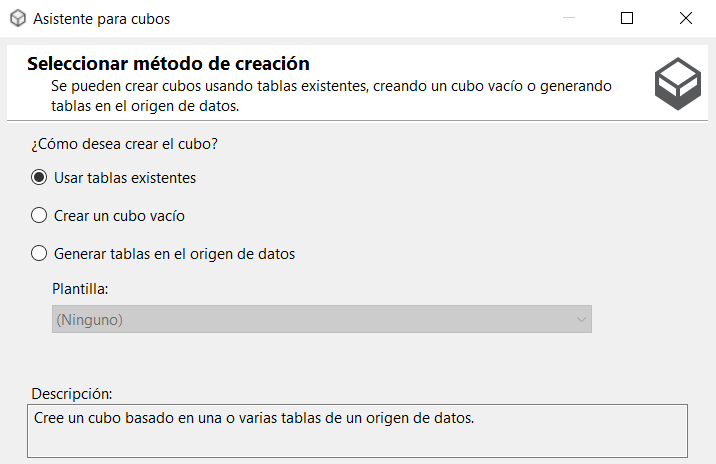
\includegraphics[width=0.75\textwidth]{image/crearCubo}
	\caption{\textbf{Creación de nuevo cubo}}
	\label{fig:9}
\end{figure}

Luego, haremos clic en "Next" y aparecerá una pantalla como la que se muestra en la Figura \ref{fig:10}.

\begin{figure}[H]
	\centering
	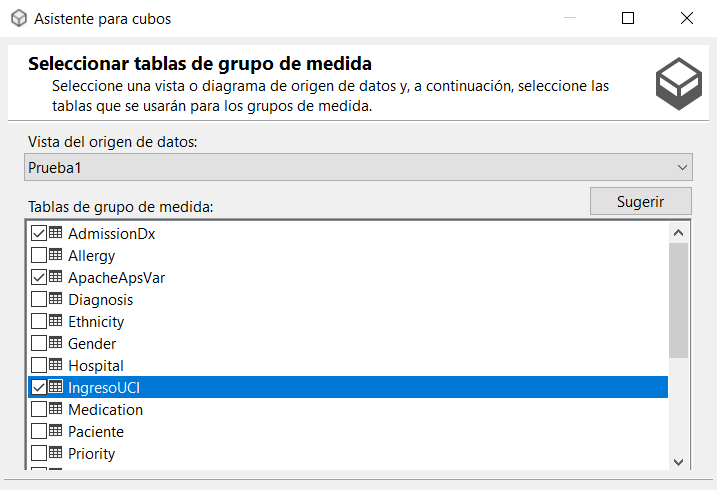
\includegraphics[width=1\textwidth]{image/seleccionTablasCubo}
	\caption{\textbf{Selección tablas del Cubo}}
	\label{fig:10}
\end{figure}

En esta pantalla, seleccionaremos únicamente aquellas \textbf{tablas que tengan una relación de tipo 1 a N} con la tabla de hechos, donde N representa las tablas relacionadas y 1 es la tabla de hechos. Esto incluye las tablas \textit{AdmissionDx}, \textit{ApacheApsVar}, \textit{RespiratoryCare}, así como las tablas intermedias (\textit{UCI\_Medicacion}, \textit{UCI\_Diagnosis} y \textit{UCI\_Alergia}) resultantes de las relaciones NxM entre las tablas \textit{Medication}, \textit{Diagnosis} y \textit{Allergy}.

Si hemos seguido correctamente los pasos anteriores, el resultado será similar al mostrado en la Figura \ref{fig:8}.

\begin{figure}[H]
	\centering
	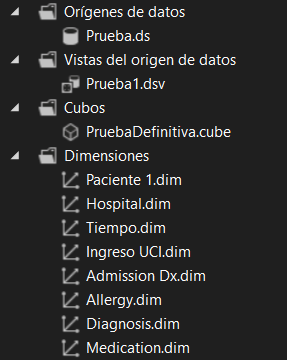
\includegraphics[width=0.5\textwidth]{image/loquellevamos}
	\caption{\textbf{Proyecto Multidimensional}}
	\label{fig:8}
\end{figure}

\textbf{Cabe destacar que las dimensiones se generan automáticamente a partir de la creación del cubo.}

	
\subsection{Modificación de las dimensiones}

Ahora procederemos con la modificación de las dimensiones para su uso correcto en el cubo.

Si damos doble clic en la dimensión \texttt{Paciente} y nos vamos al apartado de "Estructura de dimensión", veremos en la columna de atributos las claves almacenadas en \texttt{Paciente}, como se muestra en la Figura \ref{fig:11}. Ahora, lo que haremos será crear jerarquías para utilizarlas posteriormente en las consultas.

Nota: \textbf{Para cada cambio relacionado con las dimensiones, será necesario procesar y actualizar la dimensión}. Para ello, tendremos que estar en Browser o Explorador en Español.

\subsubsection{Ethnicity - Paciente}

En el caso de \texttt{Paciente}, teníamos una doble jerarquía. Por un lado, era el género y por otro, la etnia. Para crear estas jerarquías, arrastraremos la clave de la jerarquía que queramos empezar, ya sea \texttt{GenderID} o \texttt{EthnicityID}, al área donde aparece "Jerarquías". Luego, arrastraremos la clave \texttt{UniquePID}. Esto dará lugar a dos jerarquías similares a las mostradas en la Figura \ref{fig:11}.

\begin{figure}[H]
	\centering
	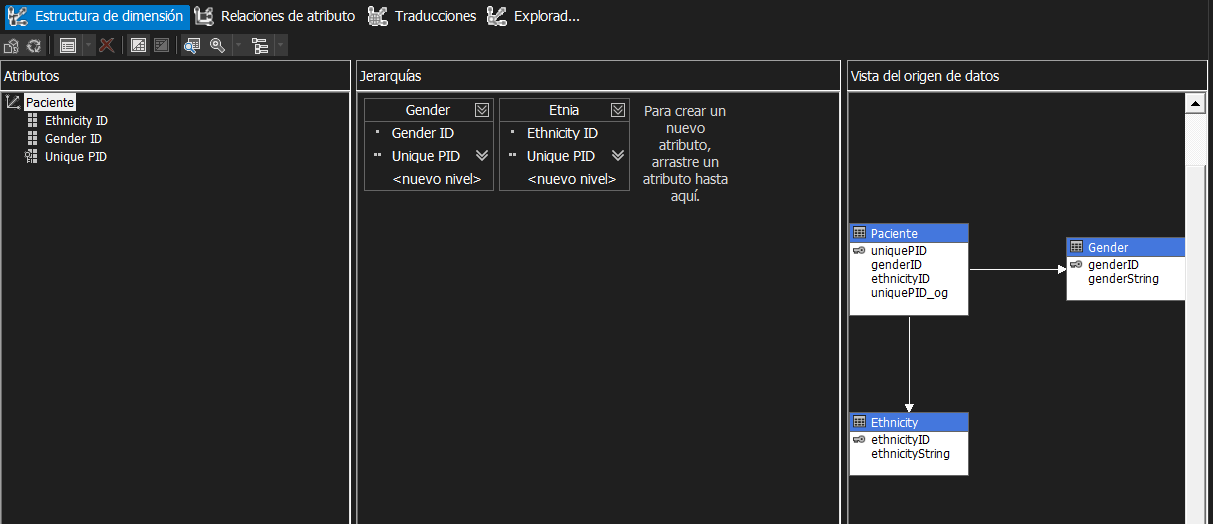
\includegraphics[width=1\textwidth]{image/dimPaciente}
	\caption{Dimensión Paciente}
	\label{fig:11}
\end{figure}

Posteriormente, para que las jerarquías se entiendan correctamente y no se utilicen solo ID's, será necesario hacer los siguientes cambios.

Daremos clic en \texttt{EthnicityID} y en el recuadro inferior derecho nos aparecerán las propiedades de dicho atributo, como se muestra en la Figura \ref{fig:12}.

\begin{figure}[H]
	\centering
	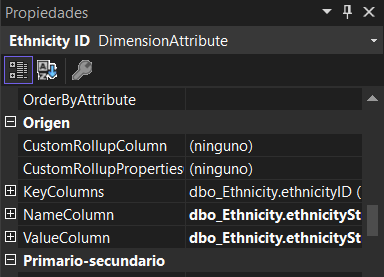
\includegraphics[width=1\textwidth]{image/EthnicityID}
	\caption{EthnicityID}
	\label{fig:12}
\end{figure}

Nos iremos al apartado \textbf{NameColumn}, le daremos a los tres puntos y nos saldrá una ventana parecida a la Figura \ref{fig:13}: 

\begin{figure}[H]
	\centering
	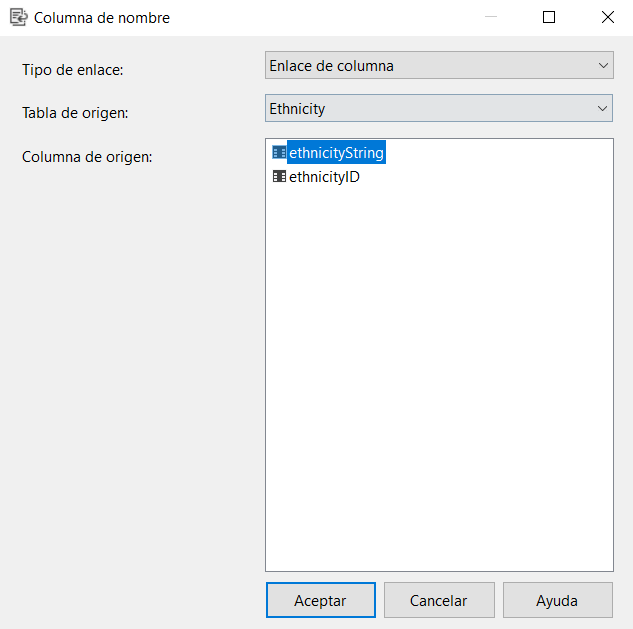
\includegraphics[width=1\textwidth]{image/EthnicityID2}
	\caption{EthnicityID}
	\label{fig:13}
\end{figure}

Ahora seleccionaremos \texttt{ethnicityString} como \textbf{NameColumn}. Ya por último, siguiendo en el apartado de propiedades, tendremos que poner en \textbf{ValueColumn} el valor \texttt{ethnicityString}, también, ya que no queremos realmente que las jerarquías sean por el ID sino por el string asociado a ellos.

Haremos exactamente el mismo proceso para el resto de tablas, \textbf{exceptuando Tiempo}, que la comentaré más tarde.

\subsubsection{Gender - Paciente}

\textbf{ValueColumn} y \textbf{NameColumn}:

\begin{figure}[H]
	\centering
	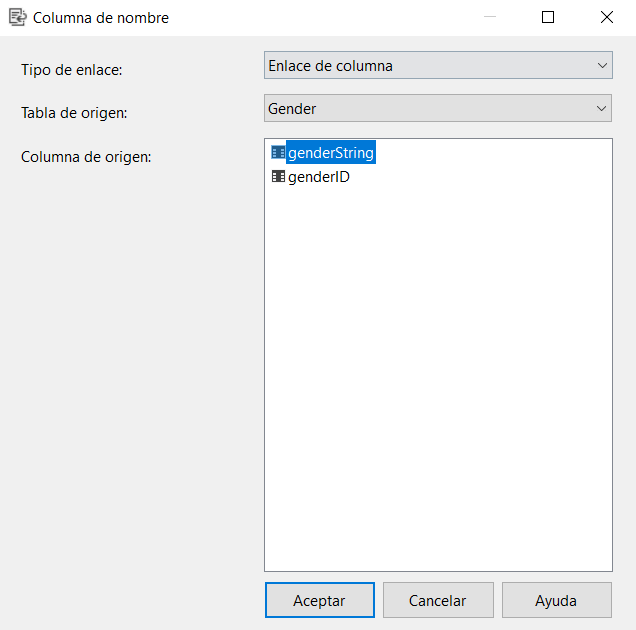
\includegraphics[width=1\textwidth]{image/GenderID}
	\caption{GenderID}
	\label{fig:14}
\end{figure}

Seleccionamos \texttt{genderString}. Al igual que antes esto es un paso "opcional" pero que mejora la calidad de nuestro cubo, si se ha probado desplegar el cubo sin cambiar estos puntos, dará resultados y se podrá hacer consultas, el problema es que estas serán más confusas, donde en lugar de hacer consultas con una etiqueta como podría ser ".male" sería correspondiente al id autogenerado para male, que vendría a ser un número que no refleja correctamente su uso.

\subsubsection{Hospital}

En el caso del hospital al ser parecido al caso anterior se empezará a obviar pasos para evitar redundancia, siendo las principales selecciones:

\textbf{Jerarquía:} Se asigna que los hospitales tengan otro nivel donde se puedan organizar según la región del hospital.

\begin{figure}[H]
	\centering
	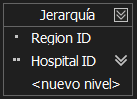
\includegraphics[width=0.5\textwidth]{image/JRegion}
	\caption{Jerarquía de Region}
	\label{fig:15}
\end{figure}

\textbf{ValueColumn} y \textbf{NameColumn} son cambiados por su versión en string que de mayor contexto.

\begin{figure}[H]
	\centering
	\includegraphics[width=1\textwidth]{image/RegionID}
	\caption{RegionID}
	\label{fig:16}
\end{figure}

En otras bases de datos el nivel más bajo de granularidad probablemente cuente con su respectivo String, como puede ser en los almacenes de comercio donde los productos, empresas, tiendas, etc. Tienen sus nombres. En el caso de la salud contamos con el inconveniente de la sensibilidad de los datos, llegando a tener el RegionString que indica la zona del hospital, pero de los hospitales solo se cuenta con los IDs asociados, que vendrían a ser un número autogenerado, al no contar con sus nombres solo se podrá cambiar los nombres del nivel de región.

\subsubsection{IngresoUCI}

\textbf{Jerarquía:}

\begin{figure}[H]
	\centering
	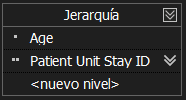
\includegraphics[width=0.65\textwidth]{image/JIngresoUCI}
	\caption{Jerarquía de IngresoUCI}
	\label{fig:17}
\end{figure}

En este nivel se tomo la decisión de tomar la edad como medidas y como dimensión para dar mayor fácilidad a la hora de hacer consultas demográficas.

\subsubsection{Allergy}

\textbf{Jerarquía:}

\begin{figure}[H]
	\centering
	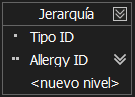
\includegraphics[width=0.65\textwidth]{image/JAlergia}
	\caption{Jerarquía de Alergia}
	\label{fig:18}
\end{figure}

\textbf{ValueColumn} y \textbf{NameColumn}:

\begin{figure}[H]
	\centering
	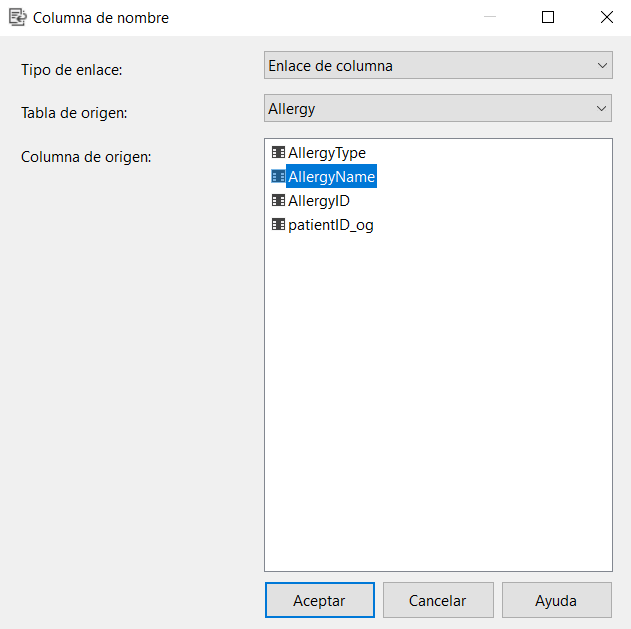
\includegraphics[width=1\textwidth]{image/allergyID}
	\caption{allergyID}
	\label{fig:19}
\end{figure}

Seleccionamos \texttt{AllergyName}.

\subsubsection{Diagnosis}

\textbf{Jerarquía:}

\begin{figure}[H]
	\centering
	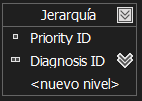
\includegraphics[width=0.5\textwidth]{image/JDiagnosis}
	\caption{Jerarquía de Diagnosis}
	\label{fig:20}
\end{figure}

\textbf{ValueColumn} y \textbf{NameColumn}:

\begin{figure}[H]
	\centering
	\includegraphics[width=1\textwidth]{image/DiagnosisID}
	\caption{DiagnosisID}
	\label{fig:21}
\end{figure}

Seleccionamos \texttt{DiagnosisString}.

\subsubsection{Medication}

\textbf{Jerarquía:}

\begin{figure}[H]
	\centering
	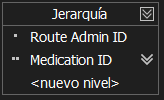
\includegraphics[width=0.55\textwidth]{image/JMedication}
	\caption{Jerarquía de Hospital}
	\label{fig:22}
\end{figure}

\textbf{ValueColumn} y \textbf{NameColumn} para \texttt{RouteAdminID}:

\begin{figure}[H]
	\centering
	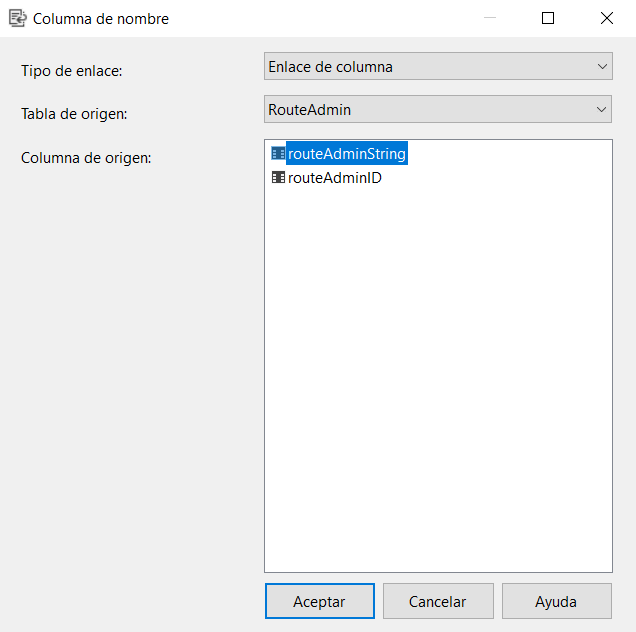
\includegraphics[width=0.88\textwidth]{image/routeAdmin}
	\caption{RouteAdminID}
	\label{fig:23}
\end{figure}

Seleccionamos \texttt{routeAdminString}.

\textbf{ValueColumn} y \textbf{NameColumn} para \texttt{MedicationID}:

\begin{figure}[H]
	\centering
	\includegraphics[width=1\textwidth]{image/MedicationID}
	\caption{MedicationID}
	\label{fig:24}
\end{figure}

Seleccionamos \texttt{DrugName}.

\subsubsection{Tiempo}

Para la dimensión Tiempo, será necesario primero arrastrar los atributos \texttt{HospitalDischargeTime24} y \texttt{HospitalDischargeYear} de la vista del origen de datos al apartado de atributos. Luego, arrastraremos primero \texttt{Year} y luego \texttt{Time24}, para tener dentro de los años las horas de ingreso asociadas.

Quedando algo parecido a la Figura \ref{fig:28}:

\begin{figure}[H]
	\centering
	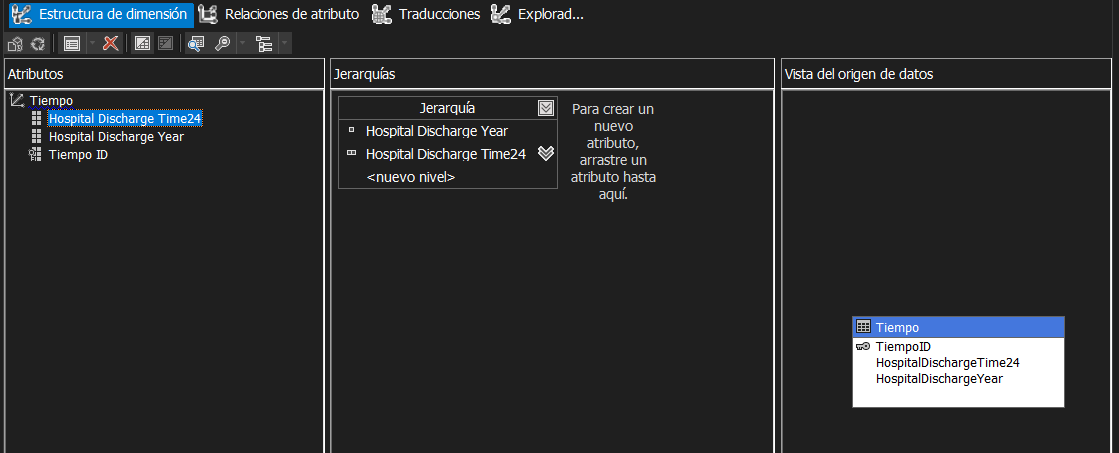
\includegraphics[width=1\textwidth]{image/JTiempo}
	\caption{Jerarquía de Tiempo}
	\label{fig:28}
\end{figure}

Posteriormente, para evitar errores de valor duplicado en la hora, haremos lo siguiente:

1. Daremos clic en el atributo \texttt{HospitalDischargeTime24}.

2. En el apartado de propiedades, seleccionaremos los tres puntos en \textbf{keyColumns}.

\begin{figure}[H]
	\centering
	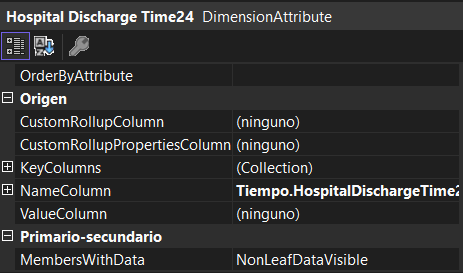
\includegraphics[width=1\textwidth]{image/tiempoPropiedades}
	\caption{Propiedades de Tiempo}
	\label{fig:25}
\end{figure}

Seleccionaremos las columnas \texttt{HospitalDischargeYear} y \texttt{HospitalDischargeTime24} para crear juntas una clave única. Con esto, aunque se repitan las horas, estarán vinculadas a un año, impidiendo el error de clave duplicada.

En \textbf{NameColumn}, seleccionaremos \texttt{HospitalDischargeTime24}. Esto es obligatorio, ya que en \textbf{keyColumn} tenemos dos claves y hay que especificar el nombre de la columna sobre la que trabajamos.

\begin{figure}[H]
	\centering
	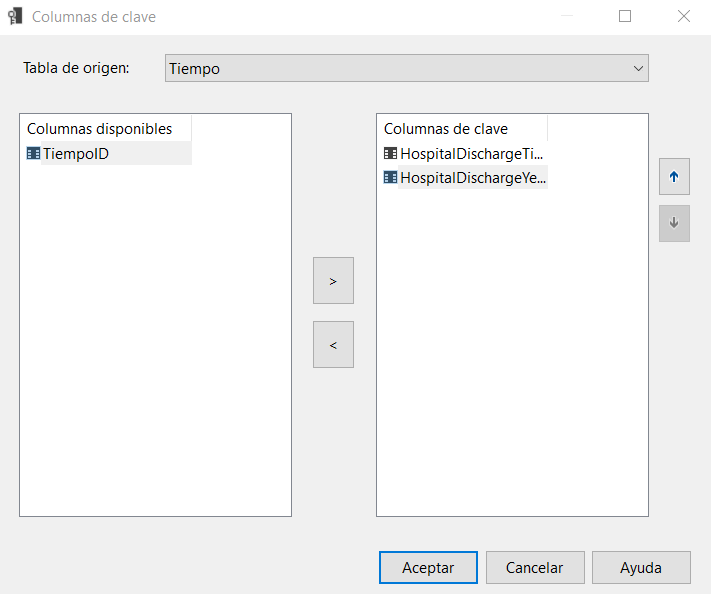
\includegraphics[width=1\textwidth]{image/keyColumnTiempo}
	\caption{Propiedades de Tiempo}
	\label{fig:29}
\end{figure}

Finalmente, en el apartado de \textbf{relaciones de atributo} dentro de la dimensión Tiempo, eliminaremos la relación entre \texttt{TiempoID} y \texttt{HospitalDischargeYear}, dando clic derecho y seleccionando "Eliminar".

\begin{figure}[H]
	\centering
	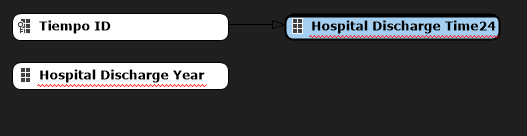
\includegraphics[width=1\textwidth]{image/relacionesTiempoDps1}
	\caption{Relaciones de Tiempo Antes}
	\label{fig:26}
\end{figure}

Luego, crearemos una nueva relación de atributo para \texttt{HospitalDischargeTime24}. Esto generará una configuración como la Figura \ref{fig:27}.

\begin{figure}[H]
	\centering
	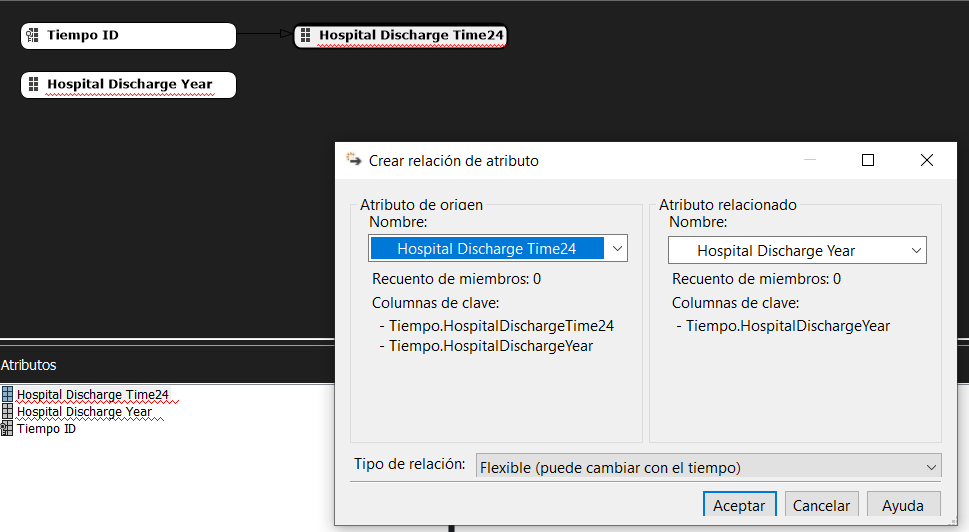
\includegraphics[width=1\textwidth]{image/relacionesTiempoDps2}
	\caption{Relaciones de Tiempo Después}
	\label{fig:27}
\end{figure}

Procedemos a darle a aceptar, y con ello habremos construido una jerarquía correctamente definida para \texttt{Tiempo}.


\subsection{Modificaciones del cubo}

Antes de proceder al despliegue del cubo, será necesario realizar ciertos ajustes en los grupos de medida para garantizar que las tablas de relación NxM funcionen correctamente. 

El ajuste principal se ilustra en la Figura \ref{fig:30}, en la cual será necesario asociar el hecho \textbf{Ingreso UCI} a la tablas  las tablas \textbf{Allergy}, \textbf{Diagnosis} y \textbf{Medication} mediante una relación de tipo varios a varios utilizando sus tablas intermedias correspondientes.

\begin{figure}[H]
	\centering
	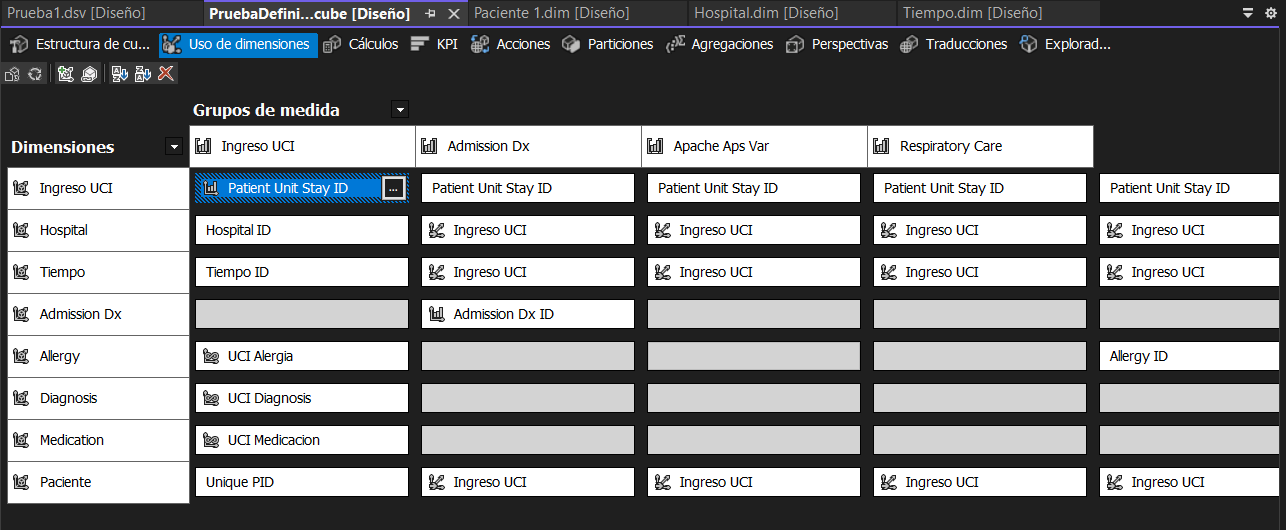
\includegraphics[width=1\textwidth]{image/gruposMedida}
	\caption{Grupos de Medida}
	\label{fig:30}
\end{figure}

\textbf{Allergy}, \textbf{Diagnosis} y \textbf{Medication} no tienen relaciones con el resto de tablas, por lo que el resto de columnas que no sean IngresoUCI o las tablas intermedias, deberán quedar vacías.

Adicionalmente, será necesario asignar \textbf{Allergy ID} como atributo de granularidad entre las tablas \textbf{Allergy} y \textbf{UCI\_Alergia}. Este mismo procedimiento deberá aplicarse a todas las demás tablas intermedias (UCI Diagnosis y UCI Medication en este ejemplo).

\subsubsection{Nuevas medidas}

Finalmente, procederemos a la incorporación de nuevas medidas, específicamente \textbf{Máximo Age} y \textbf{Mínimo Age}, como se muestra en la Figura \ref{fig:32}. Para realizar esta operación, basta con hacer clic derecho sobre la dimensión \textbf{Ingreso UCI}, seleccionar la opción \textbf{Crear nueva medida} y, en la ventana emergente, definir el uso como \textbf{Mínimo} o \textbf{Máximo}, según corresponda. La tabla origen para ambas medidas será \textbf{Ingreso UCI} y la columna origen será \textbf{age}.

\begin{figure}[H]
	\centering
	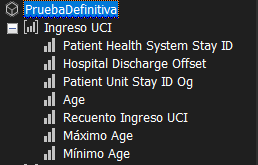
\includegraphics[width=0.7\textwidth]{image/medidasNuevas}
	\caption{Nuevas medidas}
	\label{fig:32}
\end{figure}

En este apartado se opto por usar el valor edad para probar los distintos usos que se pueden llegar a hacer en las medidas, se invita al lector a usar más de estas pues mucho tutoriales se quedan solamente con el uso de recuento cuando son herramientas que bajo ciertos contexto pueden ser útiles y fácilitar tanto la consulta o proporcionar nueva información que de otro modo llega a ser ignorada.

\subsubsection{Despliegue del cubo}

Una vez realizados todos los ajustes necesarios, el cubo estará listo para ser desplegado. El proceso se inicia pulsando el botón correspondiente, y si todos los pasos han sido ejecutados correctamente, el sistema mostrará un \textbf{check verde}, tal como se ilustra en la Figura \ref{fig:31}.

Esta medida puede proporcionar ciertos problemas al haber conexiones entre la base de datos y este archivo, un error muy común puede ser que dentro de las propiedades del proyecto en implementación este asignado el servidor localhost, esto se detallará más en el punto 4.5 a continuación.
\begin{figure}[H]
	\centering
	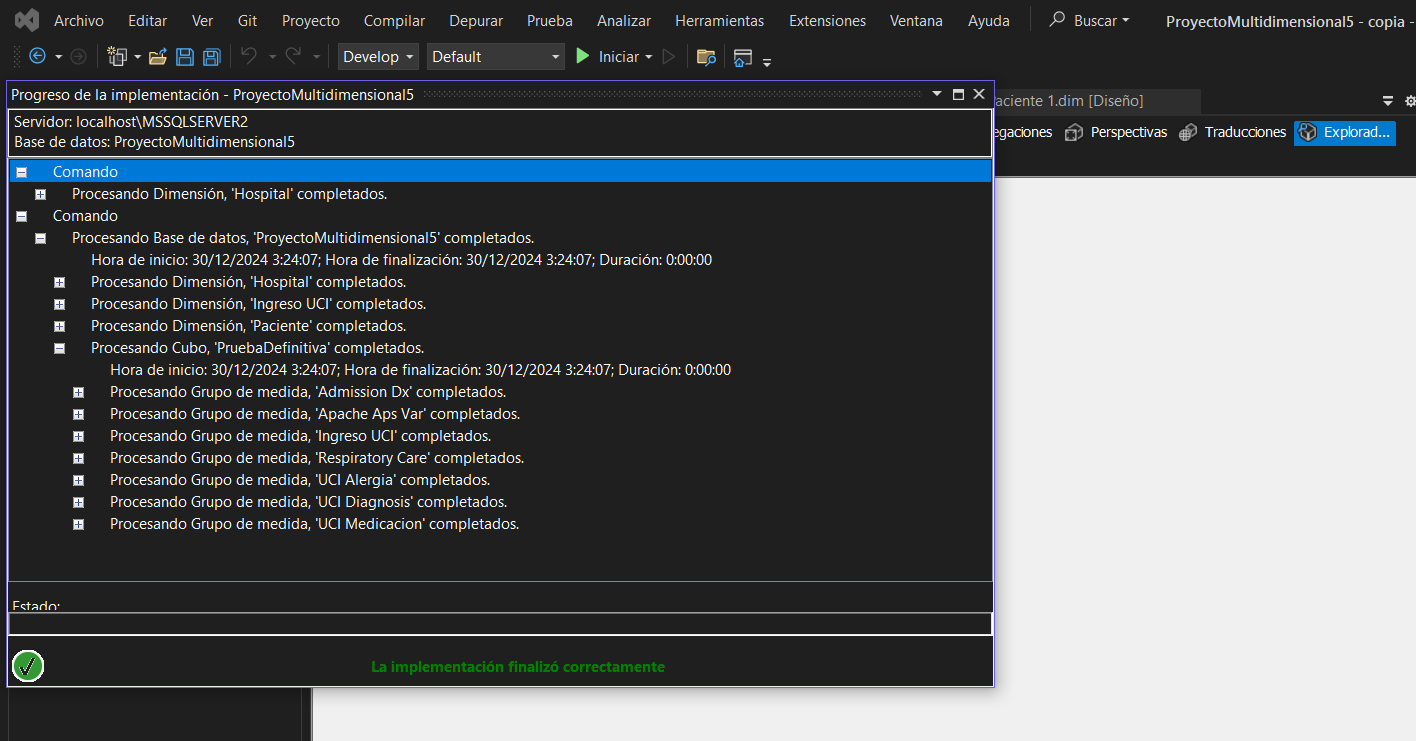
\includegraphics[width=1\textwidth]{image/checkVerde}
	\caption{Check Verde}
	\label{fig:31}
\end{figure}


\subsection{Instrucciones para desplegar el proyecto en el equipo}
	 
	 Para ejecutar la tarea, será suficiente con descomprimir el archivo. A continuación, se deberá hacer clic derecho sobre el proyecto multidimensional y seleccionar la opción ``Propiedades''. Una vez en el apartado de propiedades, se procederá a acceder a la sección de implementación, donde se deberá seleccionar el servidor correspondiente. En este caso, se podrá elegir como servidor `localhost` o bien `localhost\textbackslash nuestroServidorSQL`. En este caso particular, dado que disponía de dos instancias de `MSSQLSERVER`, fue necesario especificar que se utilizaría la instancia `MSSQLSERVER2`, que es la que posee la funcionalidad multidimensional.
	 
	 \begin{figure}[H]
	 	\centering
	 	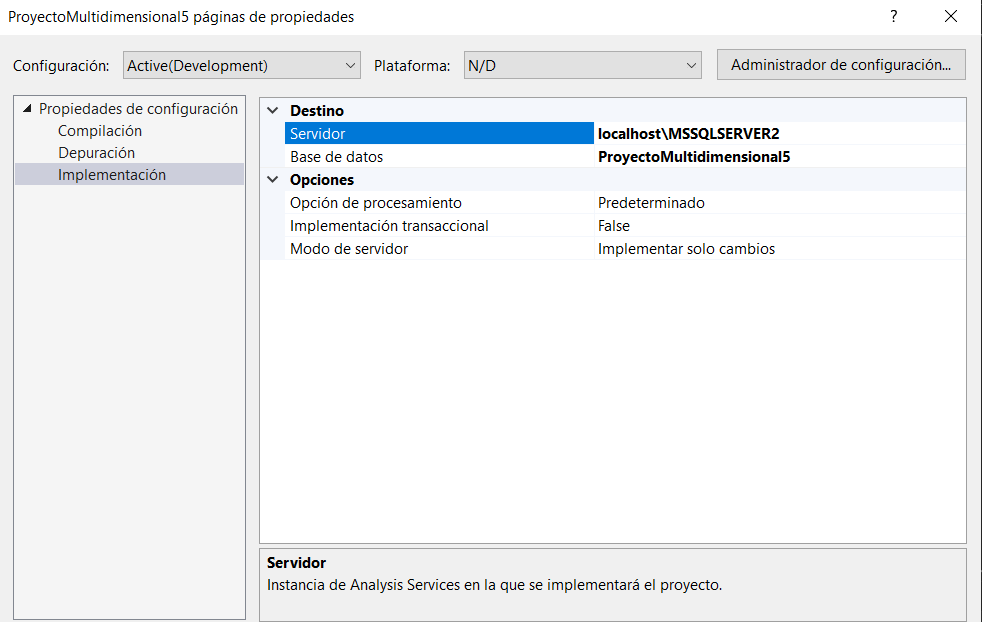
\includegraphics[width=0.75\textwidth]{image/despliegue}
	 	\caption{Configuración de despliegue}
	 	\label{fig:3}
	 \end{figure}
	 
	 Una vez configurado todo correctamente, se procederá a hacer clic en ``Iniciar'' y el proceso se completará de manera satisfactoria. 
	 
	Posteriormente, iniciaremos los servicios de Análisis (Analysis Services) en SQL Server Management Studio y verificaremos que tanto el proyecto \textit{ProyectoMultidimensional5} como el cubo se han desplegado correctamente.
	
	 
	
	\section{Consultas en MDX}
	
	A continuación, se presentan varias consultas realizadas sobre el \textit{cubo multidimensional} que contiene información hospitalaria. Se han desarrollado un \textbf{total de 8 consultas}, cuidadosamente seleccionadas para abarcar resultados de interés que respondan a preguntas clave del análisis de los datos. Estas consultas no solo utilizan \textit{funciones básicas de  MDX}, sino que también incorporan técnicas avanzadas, como medidas calculadas, filtros y agregaciones. Además, se ha hecho uso de funciones avanzadas de \textit{navegación relativa}, como \textit{PREVMEMBER, CURRENTMEMBER y PARENT}, que permiten recorrer jerarquías y explorar las relaciones entre diferentes niveles de los datos, logrando una mayor profundidad en el análisis.
	
	Cabe destacar que el cubo cuenta con el nombre \textit{PruebaDefinitiva} por practicidad, al ser un cubo desplegado a través de los datos suministrados en esta tarea comprobando su funcionamiento sin necesidad de contar con las partes anteriores, esto se resaltará más detenidamente en la siguiente sección.
	
	\subsection{Consulta 1: Total de pacientes ingresados en hospital del oeste por género y edad}
	La siguiente consulta calcula el total de pacientes ingresados en hospitales de la región oeste, mostrando además información sobre la edad media, máxima y mínima de los pacientes, agrupados por su género. Se define una medida calculada para obtener la edad media de los pacientes ingresados en la UCI.
	
	\begin{verbatim}
		WITH 
		MEMBER [Measures].[MediaEdadUCI] AS
		[Measures].[AgeTotal] / [Measures].[Recuento Ingreso UCI],
		FORMAT_STRING = "##.00"
		SELECT 
		NON EMPTY {[Measures].[Recuento Ingreso UCI], [Measures].[AgeMaximo],
			[Measures].[AgeMenor], [Measures].[MediaEdadUCI]} ON COLUMNS, 
		NON EMPTY [Paciente].[Gender ID].MEMBERS ON ROWS
		FROM 
		PruebaDefinitiva
		WHERE 
		[Hospital].[Region].[Region ID].West
	\end{verbatim}
	En la consulta anterior, se define la medida calculada \texttt{[Measures].[MediaEdadUCI]} para obtener el promedio de la edad de los pacientes ingresados en la UCI. Se realiza una agregación de las dimensiones de género, y se filtra por los hospitales ubicados en la región oeste (\texttt{[Hospital].[Region].[Region ID].West}). La salida de esta consulta puede apreciarse en la figura \ref{fig:consulta1}
	\begin{figure}[H]
		\centering
		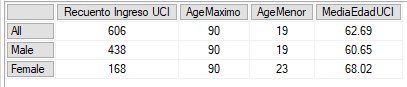
\includegraphics[width=1\textwidth]{image/consulta1.png}
		\caption{Resultado de la  \textbf{consulta 1:}  Total de pacientes ingresados en la UCI por género en hospitales de la región oeste.}
		\label{fig:consulta1}
	\end{figure}
	
	Como se puede obserar en esta región hay 606 ingresos, de los cuales podemos destacar que la mayoría son de personas masculinas, en el proceso de ETL se trato para que la edad fuera un valor \textit{int} y así poder manejarlo como una medida, en este proceso la edad correspondiente a los valores mayor que 89 fue catalogado como 90 por efectos prácticos, teniendo bastante sentido que de esta consulta tan amplia coincidan las edades máximas como mínimas. 
	
	\subsection{Consulta 2: Número de medicamentos usados por cada etnia y región de hospital.}
	
	La siguiente consulta calcula el número total de medicamentos administrados a los pacientes ingresados en la UCI, mostrando la distribución por etnia de los pacientes y la región del hospital. Se utiliza una medida calculada para nombrar con más claridad.
	
	\begin{verbatim}
		WITH 
		MEMBER [Measures].[TotalMedicamentos] AS
		[Measures].[Recuento UCI Medicacion],
		FORMAT_STRING = "##"
		SELECT
		NON EMPTY 
		{[Measures].[TotalMedicamentos]} ON COLUMNS,
		NON EMPTY [Hospital].[Region ID].MEMBERS 
		* [Paciente].[Ethnicity ID].MEMBERS ON ROWS
		FROM 
		[PruebaDefinitiva]
	\end{verbatim}
	
	En esta consulta se define la medida calculada \texttt{[Measures].[TotalMedicamentos]} para obtener el total de medicamentos administrados en la UCI. La consulta genera una tabla cruzada que combina las dimensiones de región del hospital y etnia del paciente, proporcionando un desglose detallado del uso de medicamentos por cada combinación de región y etnia. La figura \ref{fig:consulta2} muestra el resultado de esta consulta.
	
	\begin{figure}[H]
		\centering
		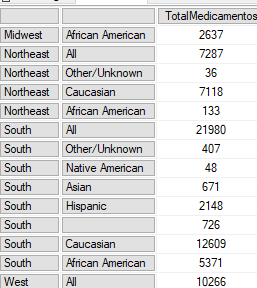
\includegraphics[width=0.65\textwidth]{image/consulta2.png}
		\caption{Resultado de la \textbf{consulta 2:}  Número de medicamentos usados por cada etnia y región de hospital.}
		\label{fig:consulta2}
	\end{figure}
	
	Es importante señalar que en esta versión de la consulta, se incluyen los grupos \texttt{ALL}, que representan todos los valores para las dimensiones de región y etnia. En el repositorio de GitHub se puede encontrar una versión alternativa de esta consulta, en la cual se excluyen los grupos \texttt{ALL}, proporcionando una versión donde se omiten las agregaciones globales.
	
	\subsection{Consulta 3: Promedio de PaO2, FiO2 y Frecuencia Respiratoria por Región Hospitalaria y Etnia para Pacientes de 20 a 30 Años en UCI}
	
	La siguiente consulta calcula el promedio de PaO2, FiO2 y frecuencia respiratoria de los pacientes ingresados en la UCI, filtrando por aquellos que tienen entre 20 y 30 años. Los resultados están desglosados por región del hospital y etnia. Además, se define una medida calculada para sumar el total de pacientes considerados.
	
	El código de la consulta 3:
	
	\begin{verbatim}
		WITH 
		MEMBER [Measures].[Total Pacientes] AS
		[Measures].[Recuento Apache Aps Var]
		MEMBER [Measures].[MediaPaO2] AS
		[Measures].[Pa O2] / [Measures].[Recuento Apache Aps Var],
		FORMAT_STRING = "##.00"
		MEMBER [Measures].[MediaFi O2] AS
		[Measures].[Fi O2] / [Measures].[Recuento Apache Aps Var],
		FORMAT_STRING = "##.00"
		MEMBER [Measures].[MediaRespiratoryRate] AS
		[Measures].[Respiratory Rate] / [Measures].[Recuento Apache Aps Var],
		FORMAT_STRING = "##.00"
		SELECT
		NON EMPTY 
		{[Measures].[MediaPaO2], 
			[Measures].[MediaFi O2],
			[Measures].[MediaRespiratoryRate],
			[Measures].[Total Pacientes]} ON COLUMNS,
		NON EMPTY 
		CROSSJOIN(
		[Hospital].[Region].[Region ID], 
		[Paciente].[Etnia].[Ethnicity ID]
		) ON ROWS
		FROM 
		[PruebaDefinitiva]
		WHERE
		([Ingreso UCI].[agePatient].[Age].&[20] : 
		[Ingreso UCI].[agePatient].[Age].&[30])
	\end{verbatim}
	
	En esta consulta se definen varias medidas calculadas, incluyendo \texttt{[Measures].[MediaPaO2]}, \texttt{[Measures].[MediaFi O2]} y \texttt{[Measures].[MediaRespiratoryRate]}, que calculan los promedios respectivos de PaO2, FiO2 y la frecuencia respiratoria. Los resultados están agrupados por región del hospital y etnia, y solo se consideran pacientes en el rango de edad de 20 a 30 años (Mediante el where). La figura \ref{fig:consulta3} muestra los resultados obtenidos.
	
	\begin{figure}[H]
		\centering
		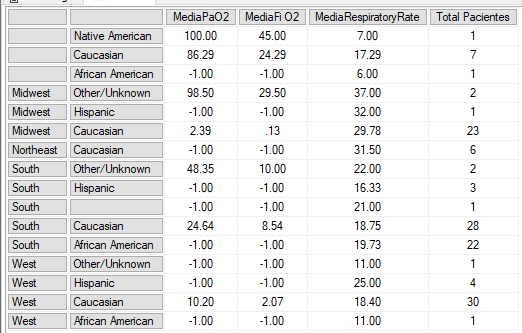
\includegraphics[width=0.8\textwidth]{image/consulta3.png}
		\caption{Resultado de la  \textbf{consulta 3:} Promedio de PaO2, FiO2 y frecuencia respiratoria por región hospitalaria y etnia para pacientes de 20 a 30 años en UCI.}
		\label{fig:consulta3}
	\end{figure}
	
	Es importante destacar que en la base de datos existen valores de \texttt{-1} que podrían indicar la ausencia de información sobre PaO2. Sin embargo, al haber valores nulos en algunas tuplas, se decidió mantener la base de datos lo más fiel posible al sistema original, ElCU, considerando que algunos médicos podrían haber registrado estos valores intencionalmente.
	
	Además, se ha observado que en algunas regiones, todos los pacientes de origen hispano y afroamericano tienen valores de PaO2 y FiO2 de \texttt{-1}, lo que no ocurre con los pacientes de origen nativo americano y la mayoría de los pacientes caucásicos. Esto podría reflejar diferencias en la calidad o disponibilidad de los registros médicos entre distintos grupos étnicos.
	
	\subsection{Consulta 4: Cálculo de Porcentaje Acumulado de Ingresos UCI por Región Hospitalaria}
	
	La siguiente consulta calcula el porcentaje acumulado de ingresos en UCI por cada región hospitalaria, excluyendo la etiqueta "Unknown" de las regiones que no contienen valores de ingresos (Esto se logra mediante Filter). Se utilizan medidas calculadas para sumar los ingresos acumulados por región y el total global de ingresos.
	
	\begin{verbatim}
		WITH 
		MEMBER [Measures].[Total Acumulado] AS
		SUM(
		{NULL:[Hospital].[Region ID].CURRENTMEMBER}, 
		[Measures].[Recuento Ingreso UCI]
		)
		MEMBER [Measures].[Total Global] AS
		SUM(
		[Hospital].[Region ID].[All], 
		[Measures].[Recuento Ingreso UCI]
		)
		MEMBER [Measures].[Porcentaje Acumulado] AS
		[Measures].[Total Acumulado] / [Measures].[Total Global],
		FORMAT_STRING = "0.00" 
		SELECT 
		NON EMPTY {[Measures].[Recuento Ingreso UCI], 
			[Measures].[Total Acumulado], 
			[Measures].[Porcentaje Acumulado]} ON COLUMNS,
		FILTER(
		[Hospital].[Region ID].CHILDREN,
		[Hospital].[Region ID].CURRENTMEMBER.NAME <> "Unknown" AND 
		NOT ISNULL([Measures].[Recuento Ingreso UCI])
		) ON ROWS
		FROM [PruebaDefinitiva]
	\end{verbatim}
	
	En esta consulta se definen varias medidas calculadas, incluyendo \texttt{[Measures].[Total Acumulado]} para sumar los ingresos en UCI por región hospitalaria, y \texttt{[Measures].[Porcentaje Acumulado]}, que calcula el porcentaje acumulado respecto al total global de ingresos en todas las regiones. Además, como se comento se uso un filtro para excluir la región "Unknown" y aquellas filas donde no existen ingresos registrados. La figura \ref{fig:consulta4} muestra el resultado de la consulta.
	
	\begin{figure}[H]
		\centering
		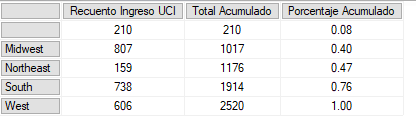
\includegraphics[width=0.8\textwidth]{image/consulta4.png}
		\caption{Resultado de la consulta 4: Cálculo de porcentaje acumulado de ingresos UCI por región hospitalaria (sin Unknown).}
		\label{fig:consulta4}
	\end{figure}
	
	Como se puede observar estamos tratando con los 2520 ingresos de la base de datos ElCU, se puede ver como se va pasando desde aquellos hospitales que no tienen una ragión asignada, a \textit{Midwest, Northeast, South} y finalmente \textit{West}. Hasta conseguir el 1 que representa el 100\% de los ingresos.
	
	\subsection{Consulta 5: Recuento de Ingresos a UCI por Hora y Total Anual}
	
	La siguiente consulta calcula el recuento de ingresos a la UCI por hora y el total anual utilizando navegación relativa dentro de la dimensión temporal. Se utiliza la función \texttt{.PARENT} para obtener los ingresos del nivel superior (año) desde el nivel más granular (hora de alta hospitalaria).
	
	\begin{verbatim}
		WITH 
		MEMBER [Measures].[Recuento Anual] AS
		([Tiempo].[Tiempo].CURRENTMEMBER.PARENT, 
		[Measures].[Recuento Ingreso UCI])
		SELECT 
		{[Measures].[Recuento Ingreso UCI], 
			[Measures].[Recuento Anual]} ON COLUMNS,
		[Tiempo].[Tiempo].[Hospital Discharge Time24].MEMBERS ON ROWS
		FROM [PruebaDefinitiva]
	\end{verbatim}
	
	En esta consulta, la medida calculada \texttt{[Measures].[Recuento Anual]} emplea la función \texttt{.PARENT} para navegar desde el nivel de la hora de alta hospitalaria al nivel padre correspondiente, que en este caso es el año. La consulta proporciona los ingresos en UCI por hora junto con el total anual de ingresos. La figura \ref{fig:consulta5} ilustra el resultado de esta consulta.
	
	\begin{figure}[H]
		\centering
		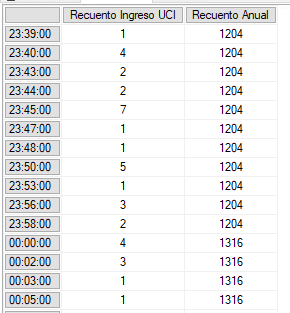
\includegraphics[width=0.8\textwidth]{image/consulta5.png}
		\caption{Resultado de la \textbf{consulta 5:} Recuento de ingresos a UCI por hora y total anual.}
		\label{fig:consulta5}
	\end{figure}
	
	El uso de la función \texttt{.PARENT} permite obtener fácilmente las medidas de un nivel superior de la jerarquía temporal, lo que es útil para calcular el total anual de ingresos en UCI mientras se observa el comportamiento a nivel de hora, esta función tiene más sentido en aquellos casos donde existen muchos niveles de granularidad como los vistos en clase.
	
	
	\subsection{Consulta 6: Recuento de Diagnósticos por Edad y prioridad en un Intervalo de Tiempo Específico (00:00:00 a 12:00:00 del 2014)}
	
	Esta consulta calcula el recuento de diagnósticos de la UCI, es decir la cantidad de diagnósticos en un intervalo de tiempo específico, entre las 00:00:00 y las 12:00:00 para el año 2014. Utiliza las dimensiones de edad y diagnóstico para obtener un desglose detallado por grupo de edad y prioridad de diagnóstico.
	
	\begin{verbatim}
		SELECT 
		{ [Measures].[Recuento UCI Diagnosis] } ON COLUMNS,
		NON EMPTY 
		CROSSJOIN(
		[Ingreso UCI].[Age].MEMBERS,
		[Diagnosis].[PriorityDiag].[Priority ID].MEMBERS
		) ON ROWS
		FROM 
		[PruebaDefinitiva]
		WHERE
		([Tiempo].[Tiempo].[Hospital Discharge Time24].&[00:00:00]&[2014] : 
		[Tiempo].[Tiempo].[Hospital Discharge Time24].&[11:40:00]&[2014])
	\end{verbatim}
	
	En esta consulta, se realiza un cruce entre las dimensiones de edad de los pacientes y las prioridades de diagnóstico, y se calcula el número de diagnósticos registrados en el intervalo de tiempo especificado. La figura \ref{fig:consulta6} muestra el resultado de esta consulta.
	
	\begin{figure}[H]
		\centering
		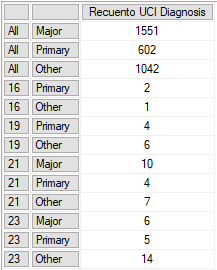
\includegraphics[width=0.7\textwidth]{image/consulta6.png}
		\caption{Resultado de la \textbf{consulta 6:}  Recuento de diagnósticos por edad y diagnóstico en un intervalo de tiempo específico (00:00:00 a 12:00:00 del 2014).}
		\label{fig:consulta6}
	\end{figure}
	
	Es importante destacar que aunque parezcan muchos diagnósticos, se están buscando todos los diagnósticos realizados desde las 00:00 hasta las 12:00 en todo el año 2014, dando 3195 de los 24978 diagnósticos de la base de datos ElCU, donde hay ingresos sin diagnósticos como ingresos con más de un diagnóstico.
	
	\subsection{Consulta 7: Análisis de Recuento de UCI por Edad, Tipo de Alergia y Etnia con la Media de Alergia por Ingresos Ordenada en Forma Descendente}
	La consulta 7 tiene como objetivo analizar los ingresos en la UCI agrupados por la edad de los pacientes, el tipo de alergia y su etnia. Además, se calcula una medida denominada \texttt{MediaAlergiaByIngresos}, que representa la media de alergias para los pacientes del determinado grupo. Los resultados se ordenan de manera descendente según este valor, destacando las combinaciones con mayor número de alergia por persona.

	
	\begin{verbatim}
		WITH 
		MEMBER [Measures].[MediaAlergiaByIngresos] AS 
		IIF(
		[Measures].[Recuento Ingreso UCI] > 0, 
		[Measures].[Recuento UCI Alergia] / [Measures].[Recuento Ingreso UCI], 
		NULL
		), 
		FORMAT_STRING = "#,##0.00" -- Formato a dos decimales
		SELECT 
		NON EMPTY 
		{ 
			[Measures].[Recuento UCI Alergia],
			[Measures].[Recuento Ingreso UCI],
			[Measures].[MediaAlergiaByIngresos]
		} ON COLUMNS,    
		NON EMPTY 
		ORDER(
		FILTER(
		CROSSJOIN(
		CROSSJOIN(
		[Ingreso UCI].[agePatient].[Age].MEMBERS, 
		[Allergy].[TipoAlergia].[Tipo ID].MEMBERS
		), 
		[Paciente].[Etnia].[Ethnicity ID].MEMBERS
		),
		NOT ISEMPTY([Measures].[Recuento Ingreso UCI])
		),
		[Measures].[MediaAlergiaByIngresos], BDESC
		) ON ROWS
		FROM 
		[PruebaDefinitiva]
	\end{verbatim}
	
	En esta consulta, se define la medida calculada \texttt{[Measures].[MediaAlergiaByIngresos]} que evalúa la proporción de casos de alergia en la UCI frente a los ingresos. El uso de \texttt{IIF} permite manejar adecuadamente los casos en los que no hay ingresos, evitando divisiones por cero. Los resultados están organizados jerárquicamente y ordenados de manera descendente (\texttt{BDESC}), mostrando primero las combinaciones con las tasas más altas.
	
	\begin{figure}[H]
		\centering
		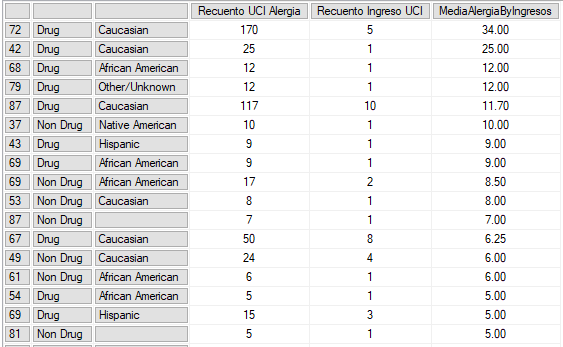
\includegraphics[width=1\textwidth]{image/consulta7.png}
		\caption{Resultado de la \textbf{consulta 7:} Análisis de UCI por edad, tipo de alergia y etnia con la media de alergias por ingresos ordenada en forma descendente.}
		\label{fig:consulta7}
	\end{figure}
	
	En la figura \ref{fig:consulta7} se pueden observar las combinaciones de edad, tipo de alergia y etnia que presentan los valores más altos de \texttt{MediaAlergiaByIngresos}. Como es el caso de la alergia a los medicamentos por parte de caucásicos de 72 años, siendo una media de 34 medicamentos a los cuales son alérgicos. 
		
	\subsection{Consulta 8: Análisis de Medicación y Parámetros Respiratorios por Género y Año, Excluyendo Pacientes de Etnia Hispánica y con Ventilación Distinta de Cero}
	
	Esta consulta realiza un análisis de medicación y parámetros respiratorios, como la media de PaO2 y FiO2, por género y año, excluyendo a los pacientes de etnia hispánica y aquellos con ventilación distinta de cero. Además, se usa la mediaPaO2 y MediaFiO2.
	
	\begin{verbatim}
		WITH 
		MEMBER [Measures].[MediaPaO2] AS
		[Measures].[Pa O2] / [Measures].[Measures].[Recuento Ingreso UCI],
		FORMAT_STRING = "##.00"
		
		MEMBER [Measures].[MediaFiO2] AS
		[Measures].[Fi O2] / [Measures].[Measures].[Recuento Ingreso UCI],
		FORMAT_STRING = "##.00"
		
		SELECT 
		{ 
			[Measures].[Recuento UCI Medicacion],
			[Measures].[MediaPaO2],
			[Measures].[MediaFiO2]
		} ON COLUMNS,
		
		NON EMPTY 
		FILTER(
		CROSSJOIN(
		[Paciente].[Gender ID].MEMBERS,
		[Tiempo].[Tiempo].[Hospital Discharge Year].MEMBERS 
		),
		[Measures].[Vent] <> 0
		) ON ROWS
		FROM 
		[PruebaDefinitiva]
		
		WHERE 
		EXCEPT(
		[Paciente].[Etnia].[Ethnicity ID].MEMBERS,
		{[Paciente].[Etnia].[Ethnicity ID].[Hispanic]}
		)
	\end{verbatim}
	
	Lo más destacable en esta función es el uso de EXCEPT que sirve para excluir a los hispanos de la búsqueda, el resto de herramientas reutilizan los visto en las demás consultas o en clase.
	
	La figura \ref{fig:consulta8} muestra el resultado de esta consulta.
	
	\begin{figure}[H]
		\centering
		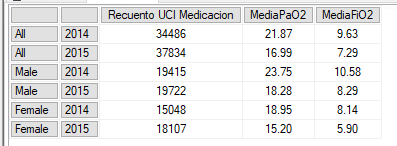
\includegraphics[width=0.8\textwidth]{image/consulta8.png}
		\caption{Resultado de la \textbf{consulta 8:} Análisis de medicación y parámetros respiratorios por género y año, excluyendo pacientes de etnia hispánica y con ventilación distinta de cero.}
		\label{fig:consulta8}
	\end{figure}
	
Los resultados tienen sentido al contar con un mayor número de pacientes masculinos como se pudo ver en la consulta 1 y en otras donde los hombres representan un grupo mayor.

\subsection{Consulta 9: Análisis del Tiempo Promedio de Alta Hospitalaria por Ruta de Medicación, Género y Diagnóstico en Pacientes de UCI}
La consulta 9 está diseñada para analizar el tiempo promedio hasta el alta hospitalaria (\texttt{Hospital Discharge Offset}) de los pacientes ingresados en la UCI, segmentado por ruta de administración de medicamentos, género y diagnóstico prioritario. Para ello, se calculan medidas derivadas que expresan este tiempo horas y días. Además, se filtran los datos para incluir solo pacientes mayores de 25 años con más de 100 administraciones de medicamentos en la UCI (al ser los pacientes que más tiempo habrán estado ingresados en la UCI), excluyendo hospitales cuya región no está asignada.

\begin{verbatim}
	WITH 
	MEMBER [Measures].[MediaHospitalDischargeOffset] AS
	[Measures].[Hospital Discharge Offset] / [Measures].[Recuento Ingreso UCI],
	FORMAT_STRING = "##.00"
	MEMBER [Measures].[MediaHospitalHORAS] AS
	([Measures].[MediaHospitalDischargeOffset] / 60),
	FORMAT_STRING = "##.00"
	MEMBER [Measures].[MediaHospitalDIAS] AS
	([Measures].[MediaHospitalHORAS] / 24),
	FORMAT_STRING = "##.00"
	SELECT 
	NON EMPTY { 
		[Measures].[Recuento Ingreso UCI],
		[Measures].[Recuento UCI Medicacion],
		[Measures].[MediaHospitalDischargeOffset],
		[Measures].[MediaHospitalHORAS], 
		[Measures].[MediaHospitalDIAS]
	} ON COLUMNS,
	NON EMPTY 
	FILTER(
	CROSSJOIN(
	[Medication].[RoutaMed].[Route Admin ID].MEMBERS,
	[Paciente].[Gender].[Gender ID].MEMBERS,
	[Diagnosis].[PriorityDiag].[Priority ID].MEMBERS
	),
	[Ingreso UCI].[Age].CURRENTMEMBER > 25
	AND [Measures].[Recuento UCI Medicacion] > 100
	) ON ROWS
	FROM 
	[PruebaDefinitiva]
	WHERE 
	EXCEPT(
	[Hospital].[Region ID].MEMBERS,
	{[Hospital].[Region ID].&[36]} --Excluyendo pacientes de hospitales cuya Region no esta asignada ""
	)
\end{verbatim}

Esta consulta incluye un poco de todo lo visto hasta el momento a excepción del tiempo total del paciente, llegando a ver pacientes con más de 10 días ingresados, como se ve en la figura \ref{fig:consulta9}
\begin{figure}[H]
	\centering
	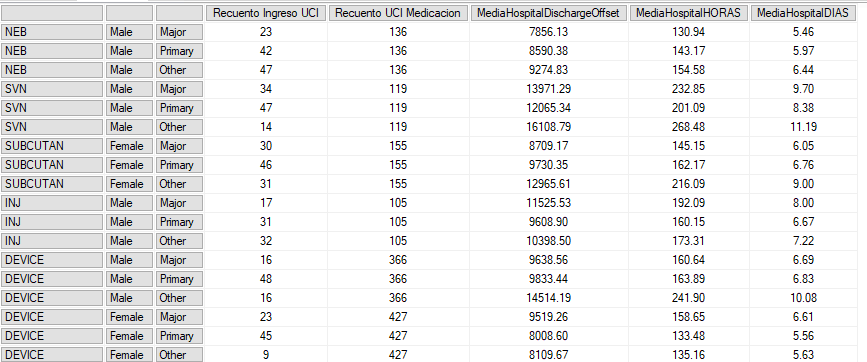
\includegraphics[width=1\textwidth]{image/consulta9.png}
	\caption{Resultado de la \textbf{consulta 9:} Análisis del tiempo promedio de alta hospitalaria por ruta de medicación, género y diagnóstico prioritario.}
	\label{fig:consulta9}
\end{figure}

Estas consultas resultan muy útiles en el ámbito médico, particularmente en el análisis de pacientes en unidades de cuidados intensivos (UCI) con patologías respiratorias. Ofrecen información detallada sobre parámetros clínicos como ingresos a la UCI, tasas respiratorias, medicación administrada y características demográficas, lo que permite identificar patrones y realizar comparaciones entre grupos de pacientes mediante filtros y cálculos específicos, como el porcentaje acumulado de ingresos por región o el análisis de parámetros respiratorios por género.

No obstante, una posible mejora sería la incorporación de datos más específicos sobre las patologías respiratorias. A pesar de que se ha realizado una transformación ETL de los datos, los valores extremos de las tasas respiratorias y de frecuencia cardíaca en la base ElCU podrían no reflejar adecuadamente las condiciones reales de los pacientes, ya que es poco probable que tantos pacientes presenten una tasa respiratoria de alrededor de 60 en situaciones de hiperventilación. Contrastar estos datos con fuentes adicionales podría proporcionar un análisis más preciso y representativo.
	
	
	\section{Instrucciones para ejecutar las consultas MDX}
	
	Para ejecutar las consultas MDX, asegúrese de que el fichero \texttt{.bak} con el almacén de datos (resultado de la tarea de ETL) y el proyecto de Analysis Services, que genera el cubo multidimensional, hayan sido desplegados correctamente siguiendo las instrucciones de los apartados anteriores.
	
	\subsection{Acceso al servidor de Analysis Services}
	Abra SQL Server Management Studio y conéctese nuevamente a la base de datos. Esta vez, seleccione el tipo de servidor como \textit{Analysis Services}. Ingrese sus credenciales como lo hizo anteriormente. Una vez conectado, expanda las bases de datos disponibles y localice la base de datos llamada \texttt{ProyectoMultidimensional5}.
	
	\subsection{Ejecución de consultas MDX}
	Para ejecutar las consultas use el botón derecho sobre el proyecto, seleccione la opción \textit{New Query} y elija \textit{MDX}. Esto le permitirá acceder al cubo \texttt{PruebaDefinitiva}. En este entorno, similar al de consultas SQL, podrá escribir y ejecutar consultas en lenguaje MDX.
	
	\subsection{Recomendaciones para la ejecución de consultas}
	Debido a la naturaleza del entorno de ejecución, solo es posible realizar una consulta por vez. Por lo tanto, se recomienda ejecutar cada consulta por separado. Si desea ejecutar varias consultas de manera consecutiva, puede cargar el archivo que contenga todas las consultas MDX. Asegúrese de seleccionar el código correspondiente a la consulta que desea ejecutar y luego presione el botón \textit{Execute} (puede ver el ejemplo en la figura \ref{fig:final}).
	
	
	\begin{figure}[H]
		\centering
		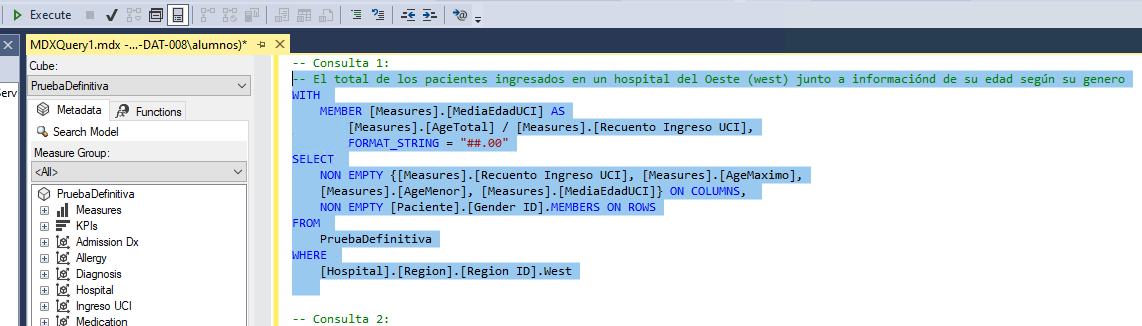
\includegraphics[width=1\textwidth]{image/final.png}
		\caption{Captura de pantalla al seleccionar una consulta juntoa l botón Execute arriba a la izquierda}
		\label{fig:final}
	\end{figure}
		
	
	\section{Problemas encontrados}

	Entre los principales problemas que encontramos, destaca la conexión con la base de datos, la cual generaba errores de manera constante debido a que el método de autenticación no estaba configurado para utilizar \textit{SQL Authentication}.
	
	Adicionalmente, surgieron problemas derivados de un proceso de ETL incorrectamente implementado, lo que resultó en la presencia de múltiples tuplas con valores duplicados, como ocurrió en la tabla \textit{ingresoUCI} inicialmente.
	
	Aunque no se considera un problema en sentido estricto, decidimos modificar el atributo \textit{age}, cambiando su tipo de dato a \textit{int} para facilitar su utilización en las consultas, dado que este atributo es de gran utilidad.
	
	La protección de datos también llega a ser un obstáculo en la comprensión y corroboración de que todo esté en orden, ya que, al contar solamente con identificadores autogenerados en la granularidad más baja, muchas veces no se podía comprobar que todo estuviera en orden a simple vista.
	
	Finalmente, destaca lo caótico que puede llegar a ser entender los errores de los programas usados, ya que contienen una gran cantidad de texto y no queda un mensaje claro sobre cuál puede ser el error. Además, se presentaron problemas con Visual Studio, que recomendaba desinstalar la extensión en casos de errores que bloqueaban la aplicación. Esto, sumado al hecho de que, en las máquinas virtuales, el servidor proxy rechazaba las conexiones, incrementó el tiempo requerido, ya que tuvimos que descargar y acceder a internet desde nuestros propios equipos.
	

	\section{Conclusiones}
	
	En esta fase del proyecto, se logró con éxito la creación de un cubo multidimensional adaptado para el análisis de pacientes con patologías respiratorias. Este cubo permite realizar consultas avanzadas que facilitan la extracción de información relevante para el ámbito hospitalario, mejorando así el análisis de datos clínicos complejos de manera eficiente.
	
	A lo largo del desarrollo, se enfrentaron varios desafíos, entre ellos, se experimento lo importante que es el proceso ETL, y como es un proceso vital que será muy útil considerar una segunda corrección una vez se empieza a desplegar el cubo y se llega a observar mejoras y necesidades en nuestro almacén, como fue el caso de la transformación del atributo \textit{Age} y la eliminación de registros duplicados. Estos ajustes permitieron desarrollar nuevas consultas en \textit{MDX} que no fueron tomadas en cuenta desde un inicio.
	
	También destacamos como una base de datos transaccional y un almacén de datos se diferencian principalmente en su propósito y estructura. Mientras que las bases de datos están diseñadas para gestionar las operaciones diarias y registrar datos de forma eficiente, un almacén de datos está optimizado para el análisis histórico y la toma de decisiones estratégicas. Un cubo multidimensional, como el implementado en este proyecto, permite la organización de datos en múltiples dimensiones, facilitando el análisis desde diferentes perspectivas, lo cual sería complejo con estructuras relacionales tradicionales. Las consultas MDX ofrecen ventajas significativas frente a SQL, al estar diseñadas específicamente para navegar y extraer información de cubos a través de varias dimensiones, permitiendo cálculos complejos y agregaciones dinámicas, algo que SQL no puede realizar de manera eficiente ni intuitiva en este tipo de estructuras, en este ejemplo de pequeña escala se puede llegar a ver, pero en caso de haber usado todo ElCU, el uso del cubo multidimensional sería aún más importante.
	
	
	Finalmente, este trabajo sienta lo aprendido y abre nuevos horizontes en cuanto a desafíos a la hora de implementar un almacén y como superarlos. 
	


	\section{Github y conjunto de instrucciones para su correcto despliegue en SQL Server.}

	Todo el proyecto está accesible en github \cite{depab2024} donde se detalla más específicamente como desplegar en SQL.
	%%%%%%%%%%%%%%%%%%%%%%%%%%%%%%%%%%%%%%%%%%%%%%%%%%%%%%%%%%%%%%%%%%%%%%%%%%%
	\printbibliography
	
	
	%% Back Cover
	
\includepdf[noautoscale=true, width=\paperwidth]{backcover.pdf}
	
\end{document}